\section{The House of Cedar, Exile, and the Open Temple}\label{sec:house-of-cedar-hidden-promise}

When Solomon brought the Ark of the Covenant out of David's tent and installed it inside the cedar-and-gold inner sanctuary of the Temple, the carrying poles were never drawn out of its rings. Pulled slightly forward, their gilded tips could be seen from the Holy Place just before the inner chamber, yet never from outside (1 Kgs 8:8). Even within the grandest house of stone and cedar Israel ever raised, those protruding staves quietly declared that the Ark was no mere static furnishing: it remained the portable throne of a pilgrim God whose dwelling among men pointed beyond walls of timber and cut stone.

\subsection{Solomon's Temple and the Resting Place of the Ark}

David had longed to build a permanent house for the Ark of God, yet the Lord reserved that work for his son Solomon (1 Kgs 6--8; 2 Chr 5--6). At the western heart of the newly raised Temple on Mount Moriah, Solomon constructed the inner sanctuary, which the Vulgate and Douay-Rheims call the ``oracle'' (\textit{oraculum}) and the Greek Septuagint of 3 Kingdoms 6:18 transliterates from Hebrew as the \textit{debir} (\textit{dabeir}):

\begin{scriptureblock}
And he made the oracle in the midst of the house, in the inner part, to set there the ark of the covenant of the Lord. Now the oracle was twenty cubits in length, and twenty cubits in breadth, and twenty cubits in height. And he covered it, and overlaid it with most pure gold. \textnormal{(1 Kgs 6:19--20)}
\end{scriptureblock}

Carved cedar paneled the Great Hall (\textit{hekal}) before it with palm trees, open flowers, and cherubim, and folding doors of olive wood opened into that windowless, unlit twenty-cubit cube (cf.\ 1 Kgs 8:12)---a geometry of complete perfection that returns in St.\ John's vision of the heavenly Jerusalem (Rev 21:16). Inside the \textit{debir}, Solomon fashioned two monumental cherubim of olive wood overlaid with gold, each ten cubits high, with wings spanning five cubits on either side---ten cubits from wingtip to wingtip (1 Kgs 6:23--26). Set side by side in the center of the twenty-cubit chamber, they stretched their wings until ``the wing of the one touched one wall, and the wing of the other cherub touched the other wall: and the other wings in the midst of the temple touched one another'' (1 Kgs 6:27--28). Above the smaller golden cherubim hammered from the Ark's own propitiatory, these towering guardians formed a golden canopy spanning the whole inner house.

In the seventh month, Ethanim, during the autumn feast of Tabernacles, Solomon summoned the elders of Israel, the princes of the tribes, and the heads of families to Jerusalem ``that they might carry the ark of the covenant of the Lord, out of the city of David, that is, out of Sion'' (1 Kgs 8:1--2; 2 Chr 5:2--3). The priests and Levites lifted the Ark together with the old wilderness tabernacle and all its sacred vessels, walking before the king and the assembled multitude, who ``sacrificed sheep and oxen, that could not be counted or numbered'' (1 Kgs 8:3--5; 2 Chr 5:4--6). Entering the darkness of the Temple, the priests set the Ark beneath the monumental wings:

\begin{scriptureblock}
And the priests brought in the ark of the covenant of the Lord into its place, into the oracle of the temple, into the holy of holies, under the wings of the cherubims. For the cherubims spread forth their wings over the place of the ark, and covered the ark, and the staves thereof above. And whereas the staves stood out, the ends of them were seen without, in the sanctuary before the oracle, but were not seen farther out, and there they have been unto this day. \textnormal{(1 Kgs 8:6--8)}
\end{scriptureblock}

That concrete eyewitness detail---preserved also in 2 Chronicles 5:9, where the ends of the staves, ``because they were some thing longer, were seen before the oracle: but if a man were a little outward, he could not see them''---confirms that the Exodus precept forbidding the poles ever to be drawn from the rings (Exod 25:15) held even inside Solomon's stone house. In Swete's Greek text of 3 Kingdoms 8:7--8, the poles are called \textit{ta hagia} and \textit{ta hegiasmena} (``its holy things'' or ``the consecrated staves''), and the concluding note ``unto this day'' is omitted.

Immediately afterward, both Kings and Chronicles record that nothing now remained inside the Ark except the two stone tablets Moses had placed there at Horeb (1 Kgs 8:9; 2 Chr 5:10). As shown in Section~\ref{subsec:contents-of-ark}, the golden pot of manna and Aaron's blossomed rod named alongside the tablets in Hebrews 9:4 belonged to the first wilderness sanctuary rather than the chest's interior four centuries later, after its captivity in Philistia and decades away from Shiloh.

As the priests emerged from the sanctuary, the Levitical singers under Asaph, Heman, and Jeduthun (\textit{Idithun}), vested in fine linen east of the altar with cymbals, psalteries, and harps alongside a hundred and twenty priests sounding trumpets, lifted one unanimous song of thanksgiving: ``Give glory to the Lord for he is good, for his mercy endureth for ever'' (2 Chr 5:11--13). At that instant the Sinai theophany returned to seal the new dwelling:

\begin{scriptureblock}
And it came to pass, when the priests were come out of the sanctuary, that a cloud filled the house of the Lord, And the priests could not stand to minister because of the cloud: for the glory of the Lord had filled the house of the Lord. \textnormal{(1 Kgs 8:10--11; cf. 2 Chr 5:13--14)}
\end{scriptureblock}

Just as Moses had been unable to enter the freshly erected Tabernacle in the desert when the cloud covered it and the glory of the Lord filled it (Exod 40:32--33 [MT/LXX 40:34--35]), so Solomon's priests stepped back before the same enveloping cloud. The dwelling of Sinai had come to rest on Mount Moriah.

\ifdefined\TriptychPrintEdition
\begin{center}
\begin{tikzpicture}
  \node[anchor=south west, inner sep=0] (image) at (0,0) {%
    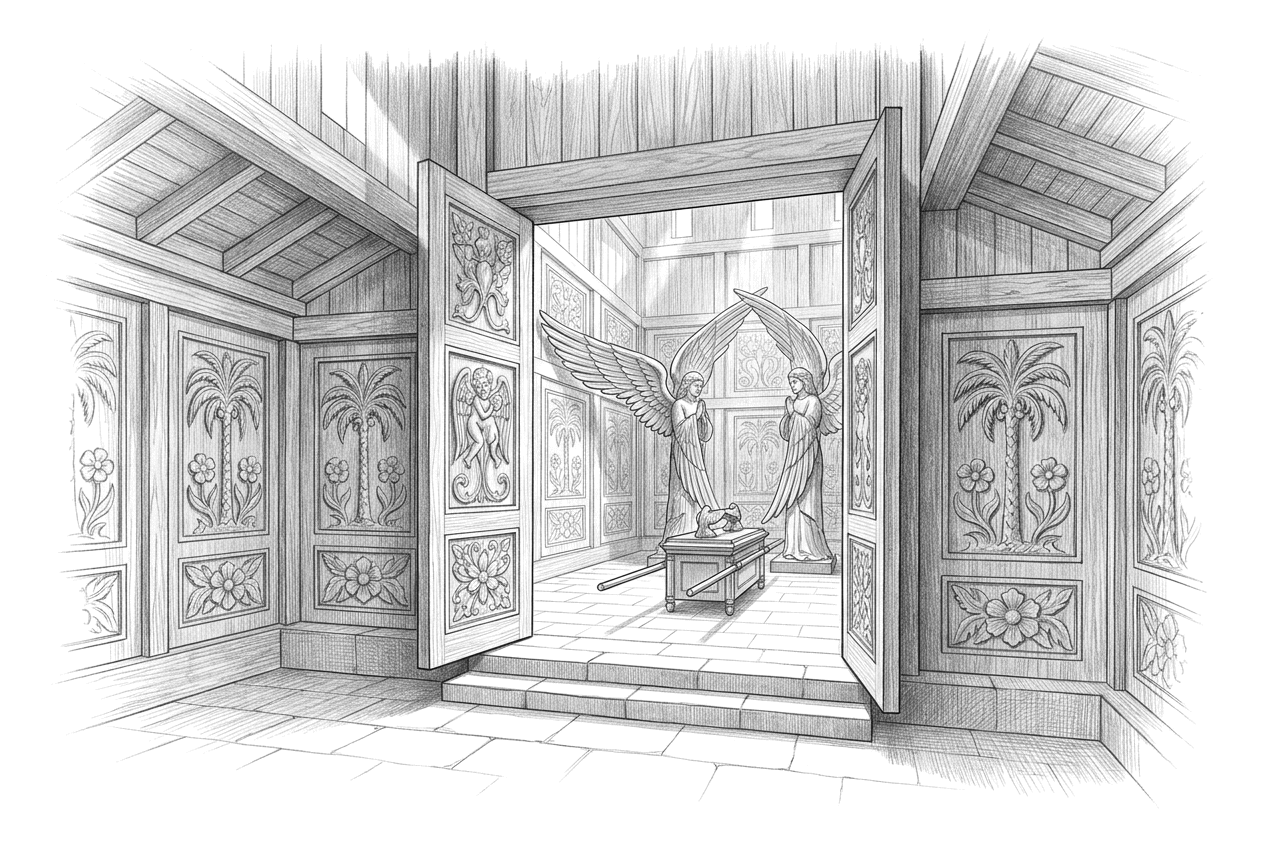
\includegraphics[width=0.92\linewidth]{theology/mariology/ark-of-the-covenant/artwork/solomon-temple-graphite.png}%
  };
  \begin{scope}[x={(image.south east)}, y={(image.north west)}]
    % Top marginal callouts in open white space above artwork
    \node[anchor=south, align=center, font=\scriptsize, fill=white, inner sep=1.5pt] (hekal) at (0.19, 1.00) {%
      Cedar-paneled Great Hall (\textit{hekal})%
    };
    \draw[line width=0.45pt] (hekal.south) -- (0.19, 0.85);
    \node[circle, fill=black, inner sep=0.9pt] at (0.19, 0.85) {};

    \node[anchor=south, align=center, font=\scriptsize, fill=white, inner sep=1.5pt] (cherubim) at (0.54, 1.00) {%
      Monumental cherubim in the \textit{debir}%
    };
    \draw[line width=0.45pt] (cherubim.south) -- (0.58, 0.66);
    \node[circle, fill=black, inner sep=0.9pt] at (0.58, 0.66) {};

    \node[anchor=south, align=center, font=\scriptsize, fill=white, inner sep=1.5pt] (doors) at (0.85, 1.00) {%
      Carved folding doors%
    };
    \draw[line width=0.45pt] (doors.south) -- (0.695, 0.80);
    \node[circle, fill=black, inner sep=0.9pt] at (0.695, 0.80) {};

    % Bottom marginal callout in open white space below floor hatching
    \node[anchor=north, align=center, font=\scriptsize, fill=white, inner sep=1.5pt] (arkpoles) at (0.55, 0.04) {%
      Ark beneath the wings; poles extending toward threshold (1 Kgs 8:6--8)%
    };
    \draw[line width=0.45pt] (arkpoles.north) -- (0.55, 0.28);
    \node[circle, fill=black, inner sep=0.9pt] at (0.55, 0.28) {};
  \end{scope}
\end{tikzpicture}
\end{center}
\else
\begin{studybox}{Plate IV: The Inner Sanctuary of Solomon's Temple}
An axial perspective looks westward from the cedar-paneled Great Hall (\textit{hekal}) of Solomon's Temple through the open double folding doors into the inner sanctuary (\textit{debir}, 1 Kgs 6:19--35; 8:6--8):
\begin{itemize}
  \item \textbf{Cedar-paneled Great Hall (\textit{hekal}):} Coffered cedar beams and carved wall panels bearing palm trees and open blossoms frame the foreground approach to the threshold.
  \item \textbf{Carved folding doors:} Tall double doors carved with cherubim, palms, and floral reliefs stand open at the top of a low stepped entrance separating the Holy Place from the Most Holy Place.
  \item \textbf{Monumental cherubim in the \textit{debir}:} Inside the twenty-cubit cube chamber, two towering sculpted cherubim stand facing forward with outstretched wings reaching from wall to wall and touching at the center above the Ark.
  \item \textbf{Ark beneath the wings and extending poles:} Resting on the stone pavement beneath the canopy of wings sits the Ark of the Covenant, crowned by its own mercy seat and bowed cherubim, with its two carrying staves projecting forward toward the doorway just as 1 Kings 8:8 and 2 Chronicles 5:9 describe.
\end{itemize}
\end{studybox}
\fi

\begin{platecaption}
\textbf{Plate IV. The Ark enthroned within Solomon's Temple (1 Kgs 6:19--35; 8:6--8).} Looking from the cedar-paneled \textit{hekal} through the carved olive-wood doors into the \textit{debir}, where the Ark rests beneath the ten-cubit gold-overlaid cherubim with its unremoved poles extending toward the threshold. Although 1 Kings 8:12 indicates that the inner \textit{debir} was an unlit chamber, the elevation uses cutaway upper light shafts purely as a drafting convention so that the monumental cherubim and the Ark remain visible. The drawing offers an interpretive architectural study faithful to the measurements and motifs of 1 Kings 6--8 and 2 Chronicles 3--5.
\end{platecaption}

\subsection{``Thou and the Ark, Which Thou Hast Sanctified'': Psalm 131 (132):8}

Solomon's prayer of dedication in 2 Chronicles 6:41 echoes a royal processional hymn that Israel sang on the ascents to Jerusalem: Psalm 131 (numbered Psalm 132 in the Hebrew Psalter). Recalling David's solemn oath to find a dwelling for the Mighty One of Jacob, the psalmist summons the pilgrims into the sanctuary:

\begin{scriptureblock}
We will go into his tabernacle: we will adore in the place where his feet stood. Arise, O Lord, into thy resting place: thou and the ark, which thou hast sanctified. Let thy priests be clothed with justice: and let thy saints rejoice. \textnormal{(Ps 131 [132]:7--9)}
\end{scriptureblock}

And the Lord answers that petition with a covenant oath over Mount Zion: ``For the Lord hath chosen Sion: he hath chosen it for his dwelling. This is my rest for ever and ever: here will I dwell, for I have chosen it'' (Ps 131 [132]:13--14).

Here a lasting divergence between the Hebrew Psalter and the Greek and Latin Bible of the Church opened an enduring theological horizon. In 2 Chronicles 6:41, every ancient textual tradition---the Masoretic Hebrew, the Greek Septuagint (Brenton), the Clementine Vulgate (\textit{tu et arca fortitudinis tuae}), and the Douay-Rheims---prays: ``Now therefore arise, O Lord God, into thy resting place, thou and the ark of thy strength.'' The Masoretic Hebrew of Psalm 132:8 preserves that exact same wording, ``thou, and the ark of thy strength'' (reflected in the Revised Version, World English Bible, and King James Version). In Psalm 131:8, however, the Greek Septuagint reads \textit{anastethi, Kyrie, eis ten anapausin sou, sy kai he kibotos tou hagiasmatos sou} (``Arise, O Lord, into thy rest; thou, and the ark of thine holiness,'' Swete and Brenton), which St. Jerome's Gallican Psalter in the Clementine Vulgate renders \textit{Surge, Domine, in requiem tuam, tu et arca sanctificationis tuae}---literally ``thou and the ark of thy sanctification,'' translated in the Douay-Rheims as ``thou and the ark, which thou hast sanctified.''

In his \textit{Commentary on the Book of Psalms}, St. Robert Bellarmine illuminates both readings side by side with admirable clarity. On verse 7 he notes the physical arrangement of the sanctuary: ``The sanctuary in the interior of the tabernacle was so constructed that the Ark was the footstool, and the propitiatory was the seat of the Lord, and was supported by two Cherubim.'' Turning to verse 8, Bellarmine explains how the psalmist invokes the infinite God in His covenant presence:

\begin{quote}\small
And he lets us see that, when he speaks thus to the Lord, he does not address him, as he essentially exists, for, as such, ``the heaven of heavens do not contain him,'' but as he is peculiarly in the Ark of the Testament, because it was from it he gave his answers, and he, therefore, adds, ``Thou and the ark which thou hast sanctified;'' that is, you and your throne, and the footstool of your feet, which footstool is ``the ark which thou hast sanctified,'' and through which you will be sanctified and honored by all who know it. In the Hebrew it is the ``Ark of thy strength,'' because it was through it God displayed his strength.
\end{quote}

Because the Septuagint and Gallican Psalter shaped the prayer of both East and West for over a millennium, that single phrase---\textit{arca sanctificationis tuae}, ``the ark of thy sanctification''---carried deep patristic and liturgical fruit. Commenting on Psalm 131(132):8, St. Augustine heard in the cry ``Arise'' the Resurrection of Christ, reading the Ark first of the Lord's own risen Body born of Mary and next of His Church rising after her Head (examined in Section~\ref{sec:fathers-liturgy}). Out of that very Christological and ecclesiological soil grew the later Eastern Dormition homilies and the Church's liturgy of the Assumption, which recognize in the Immaculate Virgin---the living Ark sanctified wholly by her Son and the personal archetype of the Church---the supreme fulfillment of the psalmist's prayer that both the Lord and the Ark of His sanctification arise together into eternal rest.

\subsection{Josiah, Jeremiah's Prophecy, and the Hiddenness of Exile}

Three centuries after Solomon's dedication, the historical books of the Old Testament mention the Ark of the Covenant for the very last time. During the solemn Passover renewal in the eighteenth year of King Josiah (621 B.C.), after the long idolatries of Manasseh and Amon had defiled the Temple courts, the reforming king issued a final command to the consecrated custodians of the Ark:

\begin{scriptureblock}
And he spoke to the Levites, by whose instruction all Israel was sanctified to the Lord, saying: Put the ark in the sanctuary of the temple, which Solomon the son of David king of Israel built: for you shall carry it no more: but minister now to the Lord your God, and to his people Israel. \textnormal{(2 Chr 35:3)}
\end{scriptureblock}

While the Hebrew, Clementine Vulgate (\textit{Ponite arcam}), and Douay-Rheims preserve Josiah's charge as an imperative, Brenton's Septuagint renders it as a completed narrative act: ``and they put the holy ark in the house which Solomon the son of David king of Israel built: and the king said, Ye must not carry anything on your shoulders.'' Whatever crisis had prompted the Levites to remove the Ark from the sanctuary during Manasseh's apostasy, Josiah returned it to Solomon's \textit{debir}. Then the historical record closes in complete silence. Thirty-five years later, when Nebuchadnezzar's armies burned the Temple of Jerusalem in 586 B.C. and catalogued the bronze pillars, lavers, firepans, and golden bowls carried off to Babylon, the Ark of the Covenant is never named among the spoils.

Yet before the flames touched Mount Moriah, the Lord had already spoken through the prophet Jeremiah an oracle that must have sounded astonishing to any Israelite who confused the wooden chest with the final goal of the covenant:

\begin{scriptureblock}
And when you shall be multiplied, and increase in the land in those days, saith the Lord, they shall say no more: The ark of the covenant of the Lord: neither shall it come upon the heart, neither shall they remember it, neither shall it be visited, neither shall that be done any more. At that time Jerusalem shall be called the throne of the Lord: and all the nations shall be gathered together to it, in the name of the Lord to Jerusalem, and they shall not walk after the perversity of their most wicked heart. \textnormal{(Jer 3:16--17)}
\end{scriptureblock}

God does not announce here that His covenant will fail, nor that He will cease to dwell among His people. Rather, He foretells a day of restoration so vast and intimate that the wooden box overlaid with gold will no longer be missed or reconstructed (``neither shall that be done any more,'' rendered ``nor will another be made'' in the World English Bible). When Jerusalem itself becomes the throne of the Lord and all nations gather to His name with healed hearts, the earthly shadow yields to a living presence that fills and surpasses what acacia wood could ever hold.

Beside Jeremiah's prophecy stands the cherished tradition preserved in the deuterocanonical second letter prefixed to the Second Book of Maccabees (composed around 163 B.C. to the Jews in Egypt, 2 Macc 2:1--8). Recalling how Jeremiah charged the exiles to keep the Law in their hearts amid the gilded idols of Babylon (2 Macc 2:1--3), the letter recounts what the prophet did with the sacred vessels of the sanctuary before the catastrophe:

\begin{scriptureblock}
It was also contained in the same writing, how the prophet, being warned by God, commanded that the tabernacle and the ark should accompany him, till he came forth to the mountain where Moses went up, and saw the inheritance of God. And when Jeremias came thither he found a hollow cave: and he carried in thither the tabernacle, and the ark, and the altar of incense, and so stopped the door. Then some of them that followed him, came up to mark the place: but they could not find it. \textnormal{(2 Macc 2:4--6)}
\end{scriptureblock}

2 Maccabees 2:4 never prints the proper name ``Nebo''; it identifies the mountain periphrastically by direct allusion to Deuteronomy 34:1, the summit from which Moses gazed across the Promised Land before his death. Rebuking those who tried to fix the location for themselves, Jeremiah uttered a promise linking the hidden Ark directly to the messianic gathering of God's people and the return of the Sinai cloud:

\begin{scriptureblock}
The place shall be unknown, till God gather together the congregation of the people, and receive them to mercy. And then the Lord will shew these things, and the majesty of the Lord shall appear, and there shall be a cloud as it was also shewed to Moses, and he shewed it when Solomon prayed that the place might be sanctified to the great God. \textnormal{(2 Macc 2:7--8)}
\end{scriptureblock}

When the exiles returned from Babylon and raised the Second Temple under Zerubbabel, no new Ark was built. For five long centuries, the Holy of Holies stood empty save for bare foundation stone---waiting for the hour when God would gather His people in mercy and reveal His dwelling anew in cloud and majesty.

\subsection{The Heavenly Temple Opened: Revelation 11:19--12:6}

Across the entire New Testament, the Greek noun \textit{kibotos} (``ark'') appears only six times: four times for Noah's ark of the flood (Matt 24:38; Luke 17:27; Heb 11:7; 1 Pet 3:20) and only twice for the Ark of the Covenant---once recalling the ancient wilderness sanctuary in Hebrews 9:4, and once piercing the veil of heaven itself in the Book of Revelation (the Apocalypse of St. John). When the seventh angel sounds his trumpet and the voices of heaven proclaim the eternal reign of the Lord and of His Christ, five centuries of silence break open:

\begin{scriptureblock}
And the temple of God was opened in heaven: and the ark of his testament was seen in his temple. And there were lightnings and voices and an earthquake and great hail. And a great sign appeared in heaven: A woman clothed with the sun, and the moon under her feet, and on her head a crown of twelve stars. And being with child, she cried travailing in birth: and was in pain to be delivered. \textnormal{(Rev 11:19--12:2)}
\end{scriptureblock}

In the Greek New Testament (across both major Greek manuscript traditions), the storm theophany of Sinai that accompanies the unveiling of the Ark includes ``and thunders'' (\textit{kai brontai}) alongside lightnings, voices, earthquake, and great hail, a phrase omitted in the Clementine Vulgate and Douay-Rheims. Even more decisive, however, is the unbroken continuity between the last verse of chapter 11 and the first verse of chapter 12. St. John wrote no chapter break here; our modern chapter divisions arose only in the late twelfth and early thirteenth centuries. Read as a single prophetic scroll, the sentence that opens the heavenly Temple and reveals the Ark of His Covenant passes without pause into the appearance of the sun-clothed Woman bearing the Messianic Child.

The Greek text stitches these verses together with tight verbal unity. At 11:19 the heavenly sanctuary opens and the Ark of His covenant ``was seen'' (\textit{ophthe}) in His temple; at 12:1 ``a great sign was seen in heaven'' (\textit{ophthe en to ourano}), the Woman clothed with the sun; and at 12:3 ``another sign was seen in heaven'' (\textit{ophthe ... en to ourano}), the great red dragon who stands poised before the Woman to devour her Child (Rev 12:3--4). The Clementine Vulgate conceals this triple Greek verb by varying its Latin equivalents---\textit{visa est} (``was seen,'' 11:19), \textit{apparuit} (``appeared,'' 12:1), and \textit{visum est} (``was seen,'' 12:3). Because the dragon of 12:3 shares the same passive verb \textit{ophthe}, the Greek formula is not an exclusively Marian marker; rather, it is St. John's unifying dramatic hinge joining the whole heavenly vision into one revelation. The Ark hidden since the Babylonian exile reappears in the opened sanctuary of heaven, and the living sign immediately unveiled in heaven is the Woman who brings forth ``a man child, who was to rule all nations with an iron rod,'' caught up to God and to His throne while she is sustained in the wilderness in a place prepared by God (Rev 12:5--6).

Eighth-century Western exegesis already read Revelation 11:19 and 12:1 as a single seamless mystery. In his \textit{Explanation of the Apocalypse}, the Venerable Bede expounds 11:19 directly of the Incarnation of the Word:

\begin{quote}\small
The temple of God, which was placed aforetime on the earth, had the ark of the covenant, inclosed within the mystical veil. But now, in the Church, which is ``the temple of the living God,'' whose ``conversation is in heaven,'' the ark of His Incarnation is laid open to the whole world, as the veil of the old temple, and the middle wall of partition, have been rent asunder by the blood of the Lord. For like the heavenly manna in clean gold is the Divinity in a holy body.
\end{quote}

Passing without interruption into chapter 12, Bede binds the opened Ark directly to the Woman: ``\textit{sign.} It is the same sign which now also appears in the Church, that God is born of man. \textit{a woman.} The Church is clothed with the light of Christ, and treads upon temporal glory.''

Catholic tradition holds these senses in harmony rather than competition. As Bishop Challoner summarizes in his note on Revelation 12:1, the Woman signifies primarily ``The church of God,'' clothed with Christ the Sun, treading the changeable things of the world beneath her feet, crowned with the twelve apostles, and laboring amid persecution to bring forth Christ in her children---yet ``It may also, by allusion, be applied to our blessed Lady.'' Only one historical Woman literally conceived and bore the male Child who rules all nations with an iron rod and ascended to the throne of God (Rev 12:5; cf. Ps 2:9), and she is simultaneously the spotless Daughter of Zion and the living archetype of the Church. For that reason, the Church's own liturgy on the Solemnity of the Assumption of the Blessed Virgin Mary (15 August) refuses to sever what St. John joined: in the postconciliar Mass during the Day, the First Reading begins deliberately at Revelation 11:19a---the opened heavenly temple and the Ark of the Covenant---and continues unbroken through 12:1--6a and 10ab, proclaiming the radiant Woman beside the Visitation Gospel of Luke 1:39--56.

\begin{threestable}{Turning Point}{Scriptural Account}{Horizon of Fulfillment}
Solomon's \textit{Debir} & 1 Kgs 6:19--28; 8:6--11; 2 Chr 5:7--14 & Ark rests beneath monumental cherubim in a golden cube; protruding poles and returning cloud show that the pilgrim Throne still points beyond stone walls.\\
\addlinespace[0.25em]
Psalm of Resting Place & Ps 131 (132):7--9, 13--14; 2 Chr 6:41 & Hebrew ``ark of thy strength'' and Greek/Latin ``ark of thy sanctification'' (\textit{arca sanctificationis tuae}) open onto Augustine's risen Body and Church and the Assumption liturgy.\\
\addlinespace[0.25em]
Josiah, Jeremiah, and Exile & 2 Chr 35:3; Jer 3:16--17; 2 Macc 2:4--8 & Last historical command in 621 B.C.; prophecy that the wooden chest will yield to a living throne; tradition of Jeremiah sealing the Ark until God gathers His people in mercy.\\
\addlinespace[0.25em]
Open Temple of Patmos & Rev 11:19--12:6 & Five centuries of Second-Temple emptiness end as the heavenly Ark appears, immediately joined across no original chapter break to the sun-clothed Woman bearing the Messianic King.\\
\end{threestable}
